% Establish the teritory, the importance and reviewing previous work. how does this assignment relate to cyber-security
\section{Introduction}

Recently in the Harvard Business Review (HBR), \textcite{Milica:2023} identified the challenges regarding cyber-security oversight by company
boards.   In the HBR report survey, boards are saying that they are not seeing eye-to-eye with their CISOs, with one example being that while
\enquote{65\% of board members think their organization is at risk of a material cyber-attack, only 48\% of CISOs share that view.}

European and US companies are spending more each year on cyber-security (having increased over 50\% in the last three years \autocite{Hiscox:2022}),
and that expectation is reflected in the HBR survey, where 87\% of board members are expecting these budgets to increase again in the next year.  

\begin{figure}[!ht] % Single column figure
  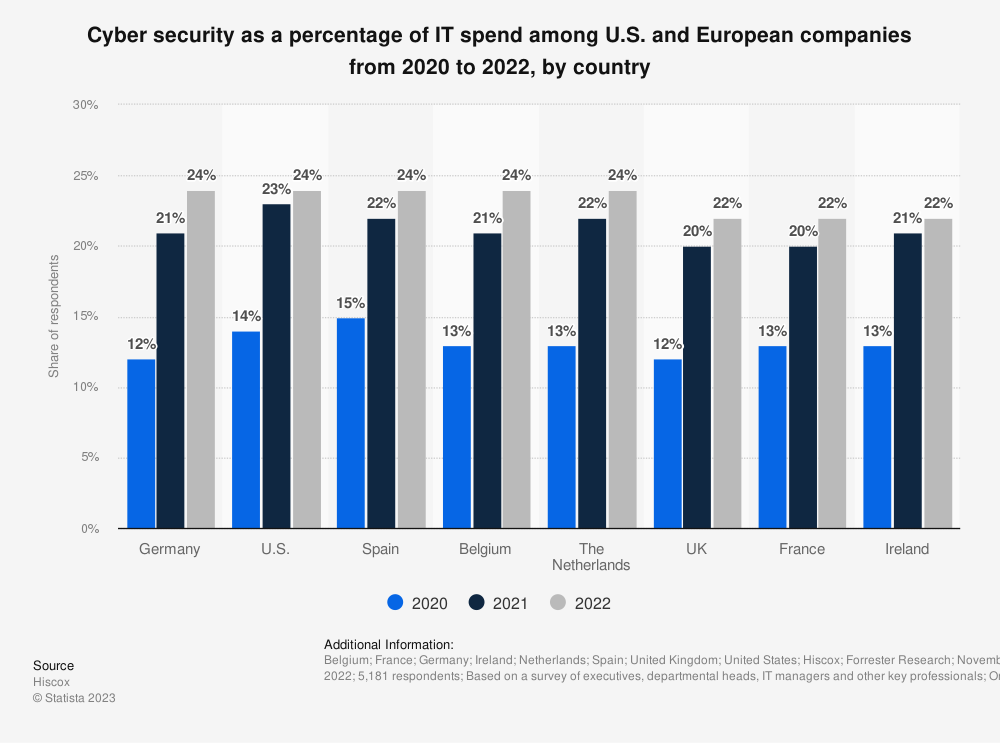
\includegraphics[width=0.95\textwidth]{statistic_id1245356_share-of-it-spend-on-cyber-security-in-the-us-and-europe-2020-2022-by-country.png}\hfill
  \caption{Spending on Cyber Security  \autocite{Hiscox:2022}  Source: Statistica Inc.}
  \label{fig:cybersecurity-spending}
\end{figure}


And the pessimism of the board members' expectations of a material cyber-attack is reflected in the reported monetary damage caused by
cyber-crime, having nearly trebled in the US over the same three-year period \autocite{FBI:2023}.  Yet the HBR reports that 76\% of
board members believe they have made adequate investments in cyber-protection.

\begin{figure}[!ht] % Single column figure
  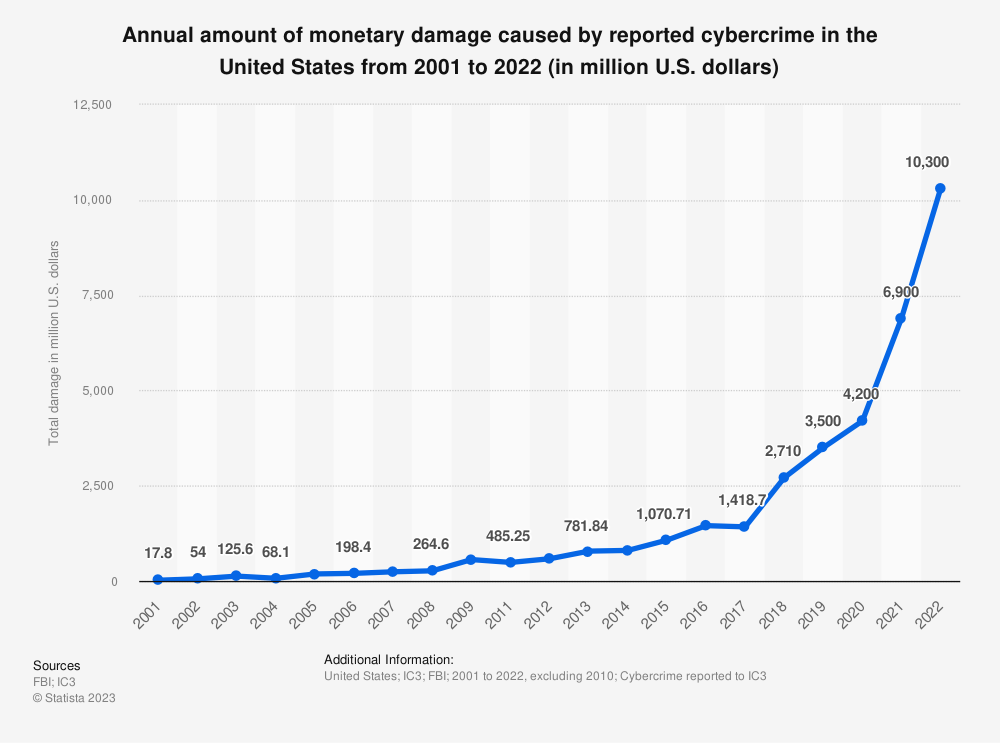
\includegraphics[width=0.95\textwidth]{statistic_id267132_annual-amount-of-financial-damage-caused-by-reported-cybercrime-in-us-2001-2022.png}\hfill
  \caption{Financial Damage caused by Cybercrime in the USA year-on-year \autocite{FBI:2023} Source: Statistica Inc.}
  \label{fig:cybercrime-cost}
\end{figure}

And there lies a key point highlighted by the report; these organisations are talking in terms of protection, not resilience.

% Identify a niche, indicating a gap in in knowledge
\subsection{Resilience vs protection}

The National Institute of Standards and Technology's (NIST) Cybersecurity Framework (CSF) \autocite{NIST:2018} continues to develop a set of baseline
cyber-security practices.  Within this set of functions, they outline:

\begin{itemize}
\item Safeguards to ensure the delivery of services [\textit{Protect}].
\item Maintenance of plans to restore services and capabilities impaired due to a cyber-event [\textit{Recovery}].
\end{itemize}
  
Using such a framework it is this reports position that it is possible to engage with this
\enquote{communication gap and board-CISO misalignment [that] hinders progress in cybersecurity}
and to make the improvements to cyber-security oversight highlighted by the HBR authors:

\begin{itemize}
\item Refocus on resilience not protection and address the contradiction between budget expectations and the perceived risk. 
\item Improve communications to ensure cyber-security is continuous priority with ongoing board commitment.
\item Make cyber-security discussions about organisational risk with a strategic imperative, not a technical topic that is difficult to engage with. 
\end{itemize}


%The life of a cyber-security professional can be a thankless task at times.
%Even with cyber-security spend increasing as a percentage of IT
%budgets \autocite{Hiscox:2022}, 

%Considering the challenges identified in the Harvard Business Review article regarding cybersecurity oversight by boards, this report seeks to address these issues and propose a strategic enhancement for Chief Information Security Officers (CISOs). The key concerns include:

%The authors went on to propose a strategic enhancement for Chief Information Security Officers (CISOs).

%\subsection{CISO Challenges in Cybersecurity Oversight by Boards}
%
%\begin{enumerate}
%\item Disconnect Between Boards and CISOs:
%     \begin{itemize}
%        \item Limited alignment between boards and CISOs.
%        \item Insufficient interaction hindering meaningful cybersecurity discussions.
%        \item Communication gaps and misalignment impeding progress in cybersecurity.
%     \end{itemize} 
%\item Focus on Protection Over Resilience:
%     \begin{itemize}
%        \item Boards prioritizing cyber protection despite a high perceived risk.
%        \item Investments in protection not directed to critical areas.
%        \item Advocacy for a shift towards organizational resilience.
%     \end{itemize} 
%\item Cybersecurity as a Technical Topic:
%     \begin{itemize}
%        \item Boards viewing cybersecurity primarily as a technical issue.
%        \item Limited time in board meetings making it challenging to address nuances.
%        \item Need for a shift from technical to management challenges in discussions.
%     \end{itemize}
%\item Board Composition and Expertise:
%     \begin{itemize}
%        \item Many boards lacking cybersecurity expertise.
%        \item SEC proposing explicit cybersecurity recommendations for boards.
%        \item Necessity for board composition changes to incorporate cybersecurity knowledge.
%     \end{itemize} 
%\item Priority and Commitment:
%     \begin{itemize}
%        \item A quarter of boardrooms not viewing cybersecurity as a priority.
%        \item Inadequate frequency of cybersecurity discussions.
%        \item The necessity of making cybersecurity a continuous priority with ongoing commitment.
%     \end{itemize}
%\end{enumerate}

%Organisations are clearly spending more on cyber-security.  Financial damage is going up. But the HBR report highlights a focus on prevention rather than resiliency.  
   
%\subsection{The CISO and current state of malware attacks on Windows.}

%\textbf{Importance of addressing issues in cybersecurity oversight by boards}.

%To address these challenges, this report proposes a strategic proposition aimed at enhancing the CISO's position within the organization. The proposition includes:
%\begin{enumerate}
%      \item Engagement with Senior Executives:
%         \begin{itemize}
%            \item Demonstrating the importance of cybersecurity as an organizational imperative.
%            \item Building personal relationships with senior executives to bridge the communication gap.
%         \end{itemize}
%      \item Explanation of Cyber-Resilience Program:
%         \begin{itemize}
%            \item Clearly communicating the organization's cyber-resilience strategy.
%            \item Translating technical jargon into business language for better understanding by the board.
%         \end{itemize}
%      \item Initiatives within the Department:
%         \begin{itemize}
%            \item Developing regular cybersecurity reports to provide transparent insights.
%            \item Showcasing the department's efforts in enhancing cyber resilience.
%         \end{itemize}    
%      \item Use Case Report on Process Injection Attacks:
%         \begin{itemize}
%            \item Presenting a real-world use case demonstrating new process injection attacks.
%            \item Evaluating the effectiveness of the organization's Endpoint Detection Response system (EDR).
%         \end{itemize}         
%      \item Ensuring EDR Vendor Adaptation:
%         \begin{itemize}
%            \item Using the use case report to ensure the EDR vendor is adapting to new threats.
%            \item Strengthening the organization's defence mechanisms against evolving cyber threats.
%         \end{itemize}
%\end{enumerate}


%This comprehensive approach aims not only to address the challenges outlined in the Harvard Business Review article but also to elevate the CISO's role by fostering better understanding, engagement, and preparedness within the organization. cite \href{https://www.cisa.gov/cross-sector-cybersecurity-performance-goals}{cross-sector-cybersecurity-performance-goals} and 



%Relying on EDR systems as a principle defence against a myriad of attacks alieviates many problems.  But it does not alievate the communication gap between company boards
%and the cyber and information security professionals that protect their organisation.  CISOs need to understand the threat landscape, their mitigants to attacks, and
%where failures in their own security systems may fail.  Having new internal analysis and being fully abreast of the threats, vulnerabilities and mitigants of their
%systems will equip our CISO with the information they need to formulate and communicate a set of action/response readiness to the senior executives and board members.
%\subsection{Introducing Mockingjay: Importance of understanding process injection techniques.}
%This cat-and-mouse game beween security groups on the one hand, and the evasion and increased sophistication and novelty on the part of malicious actors on% the other \ldots
%\textit{introduce EDR} \ldots
%For vendors of EDR, MDR \& XDR solutions investigating existing and emerging threats is an on-going process \href{https://research.tue.nl/files/305661196/Olteanu_I.C..pdf}{evaluating the response effectiveness of their XDR technology}.

% Occupy the niche; purpose of new research, listing questions, the value of the work and the structure of the writing


\subsection{Turning a threat into a strategic enhancement for the CISO}

This paper presents a model for the type of analysis that a CISO should be requesting from their information security teams.

Process Injection (PI) is a technique to dynamically modify a running process to introduce some new functionality.  It is used by malware and virus coders to
deliver, and execute, a malicious payload into the addressable memory space of a legitimate process.  This is engineered to be done without
being detected by anti-virus software or other defensive systems. 

End-point Detection and Response (EDR) is an integrated security solution that uses real-time continuous monitoring of processes and systems, and the data generated from these systems, to detect malware either directly, or through anomalous behaviour of the monitored systems.

This paper reports on a new process injection technique named ``Mockingjay'' \autocite{Peixoto:2023} that seeks to evade the protections offered by EDR technologies.  We will investigate the attack in a case study produced by a cyber-security group in a hypothetical organisation and couch the response
to address all NIST CSF functions and include resilience as a core part of the response to the threat.

%, and specifically with behaviours that could be used to detect API attacks \autocite{Wang:2022}.

%We will analyse the ``Mockingjay'' attack and identify the defences offered by modern XDR systems and ask if there's a credible chance of evading detection.  By looking at an implementation of the attack we will ask in what ways a threat detection system strengthen it's defences, and what artifacts could be automatically produced that could demonstrate any anomoly in a systems behaviour. 

Section 2 is a overview of changing landscape of threat actors and defence mitigants.  We review process injection methods, focusing in on file-less exploits leveraging the Windows system used by Mockingjay.  We also look at how malware detection has adapted to these threats and examine end-point protection such as EDRs.

%We will then look at methods a identifying these attacks and look at the likelihood of Endpoint Security products of identifying the attack.   An investigation into the Mockingjay attack and against a recently published paper ``Procguard'' \autocite{Wang:2022} and asks whether this attack method would lickly be caught.

Section 3 is the case study on the Mockingjay process injection attack that a CISO should be expecting from their team.  It will demonstrate that
every analysis that the cyber-security team undertakes can be an opportunity to safeguard critical services and ensure that services can be
restored from as successful attack.

%crystalise challenges
%that our titular CISO should be engaging his vendor on.  It should also feed back into the cyber-security playbooks that the organisation has, and
%the threat and response reported back to senior executives and boards.

%to use reinforcement to identify ``RWX'' code injections that should be part of a corporations EDR solution.
% {jwang,mcj123,ZiangLi,2018302180148,iwangjye}@whu.edu.cn

%Section 5 is an implementation of the attack and will look at manually identifying an infected process and generating artifacts that could be used in automating the process.

Section 4 is the conclusion where we highlight how taking a holistic view when understanding threats and threat actors can help build more
resilient cyber-security systems and define the CISO function as an important strategic foundation for mitigating operational risks.

Section 5 is a reflection on the project outcomes.

%and will suggest risks and mitigants for process injection attacks and further research that could be undertaken to adapt to and mitigate evolving cyber-security threats.